\chapter{Supplementary Figures}\label{app:figures}

This appendix collects supplementary diagnostic figures whose
chapter-five renderings are referenced from the main text and whose
larger format is deferred here for readability. Each figure is paired
with a brief caption summary; the underlying data tables are stored
alongside the figures in the repository under
\texttt{Master\_Thesis/figures/chapter5/}.

\section{DHO rotation angle and viscosity diagnostics}\label{app:figures:dho}

The DHO mechanism's per-block rotation angle $\theta_{t, h, b}$ and
its per-head per-block viscosity coefficient $\eta_{h, b}$ are the
two diagnostic scalars that determine whether the mechanism is
exercising its physical-prior structure. The supplementary
visualisation in Figure~\ref{fig:app:dho-eta-theta} plots the
per-layer realised distribution of $\theta$ alongside the trained
$\eta$ values at the close of training, taken across the matrix's
DHO cells. The figure is rendered from the per-cell diagnostic
checkpoints under \texttt{experiments/final/outputs/<cell>/}; the
data table is
\texttt{F9\_dho\_eta\_theta\_data.csv}, and the rendering script is
\texttt{F9\_dho\_eta\_theta\_script.py}.

\begin{figure}[h]
\centering
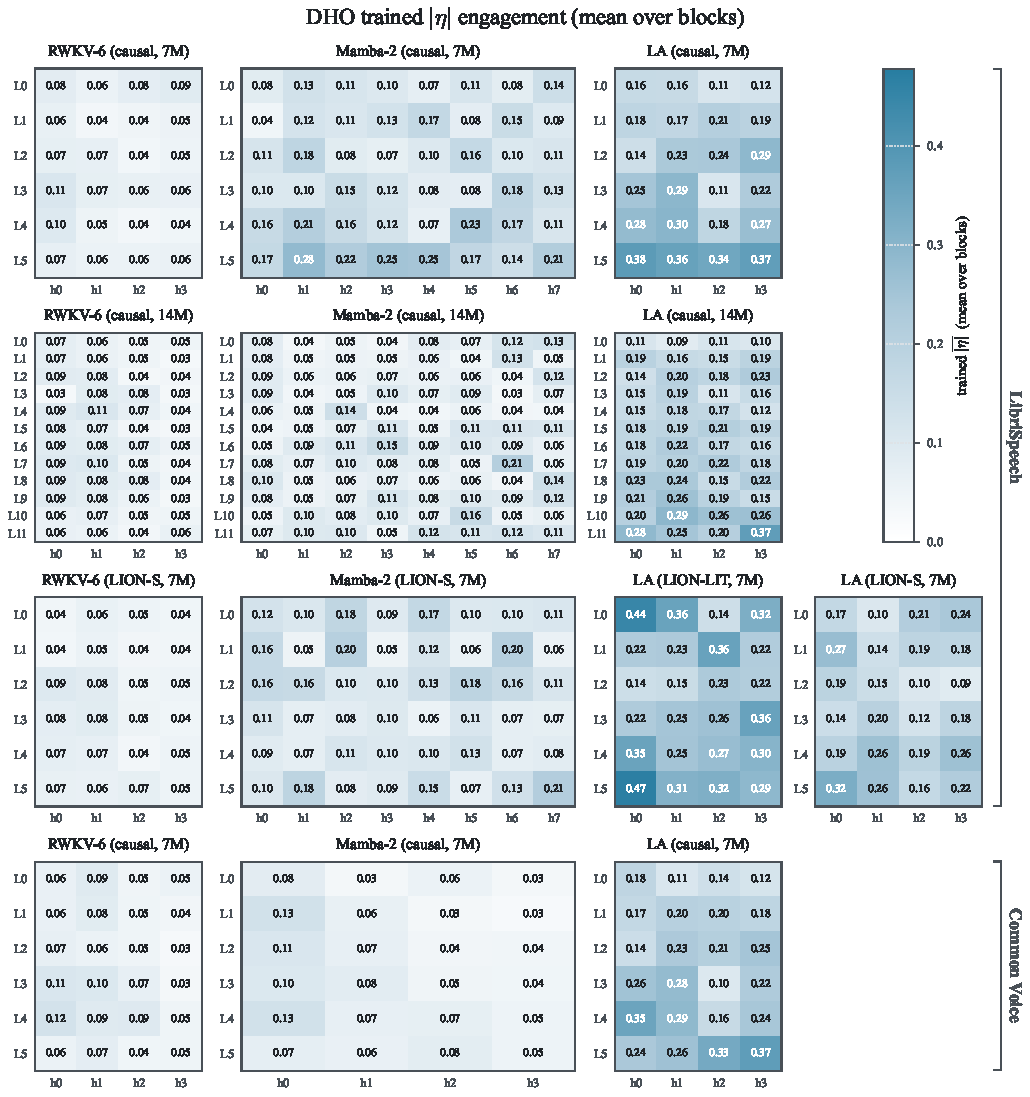
\includegraphics[width=0.95\linewidth]{chapter5/F9_dho_eta_theta.pdf}
\caption[DHO eta-theta diagnostic]{Per-layer rotation-angle and
viscosity-coefficient diagnostics for the DHO cells in the matrix.
The depth-graded $\theta$-clip schedule is visible in the
right-hand panel; the trained $\eta$ values exhibit
architecture-specific signs that align with each backbone's
structural deficit (Section~\ref{sec:dho-mechanism-engagement}).}
\label{fig:app:dho-eta-theta}
\end{figure}

\section{CVD per-head temperature heatmaps}\label{app:figures:cvd}

The CVD mechanism's per-head learnable temperature $\tau_{h}$ is
the load-bearing free parameter of the chunk-local preconditioner.
Figure~\ref{fig:app:cvd-tau} plots the trained $\tau_{h}$ values per
layer and per head across the productive CVD deployments. The
underlying data table is \texttt{F10\_cvd\_tau\_heatmaps\_data.csv}.

\begin{figure}[h]
\centering
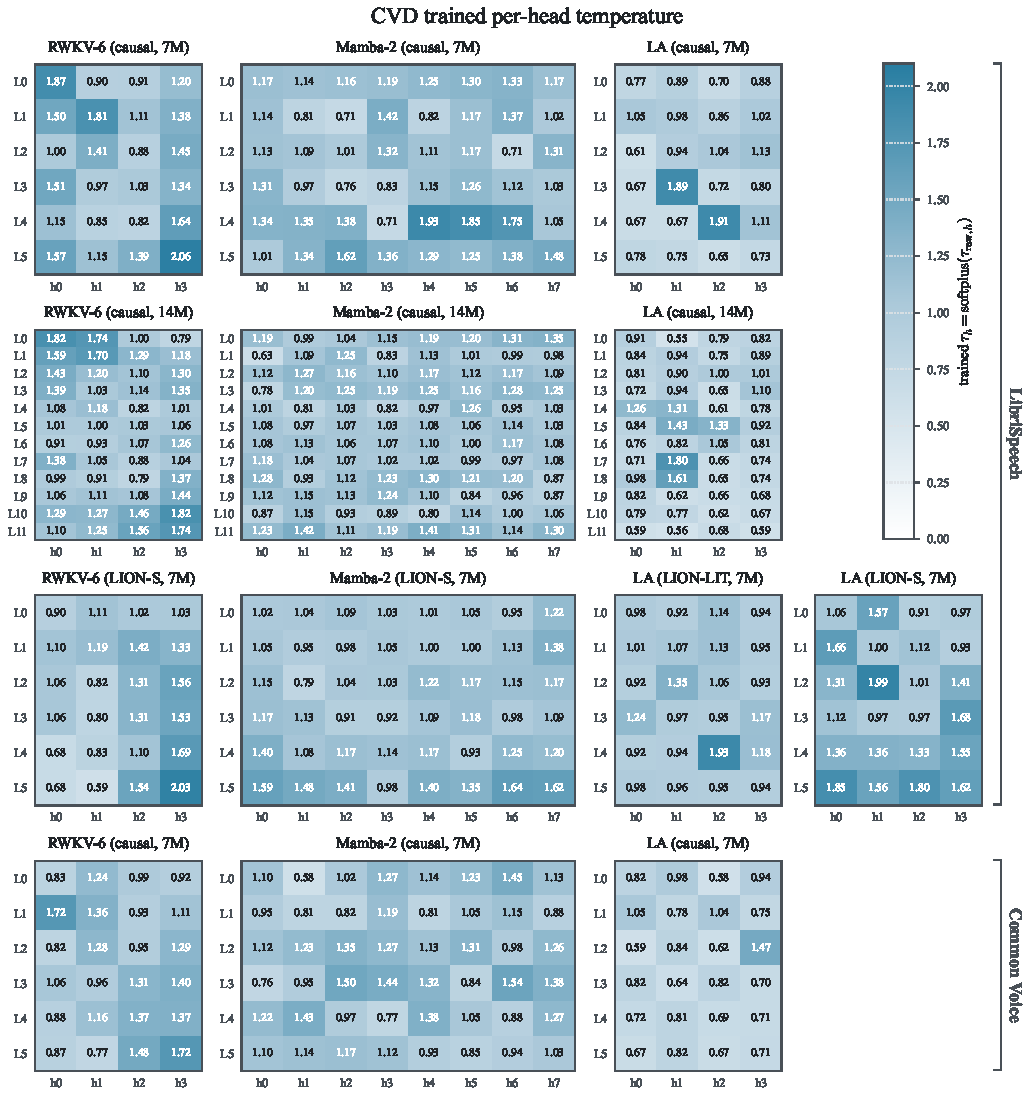
\includegraphics[width=0.95\linewidth]{chapter5/F10_cvd_tau_heatmaps.pdf}
\caption[CVD per-head temperature heatmaps]{Trained $\tau_{h}$ values
per layer and per head across the productive CVD deployments. The
across-architecture heatmap pattern exhibits substantial
between-head variation, confirming that the per-head temperature is
exercised by the gradient and that the mechanism's per-head
freedom is not redundant.}
\label{fig:app:cvd-tau}
\end{figure}

\section{Per-cell training curves}\label{app:figures:training-curves}

The per-cell training curves on the matched 50-epoch budget are
plotted in Figure~\ref{fig:app:training-curves} as a small-multiples
grid. Each panel shows dev CER as a function of epoch for a single
cell of the LibriSpeech matrix. The grid is intended for visual
verification that the matched-budget convergence horizon is not
truncated and that no reported cell exits the patience-15 early
stopping criterion before the 50-epoch budget completes. The
underlying per-epoch records are
\texttt{history.csv} files under
\texttt{experiments/final/outputs/<cell>/}.

\begin{figure}[h]
\centering
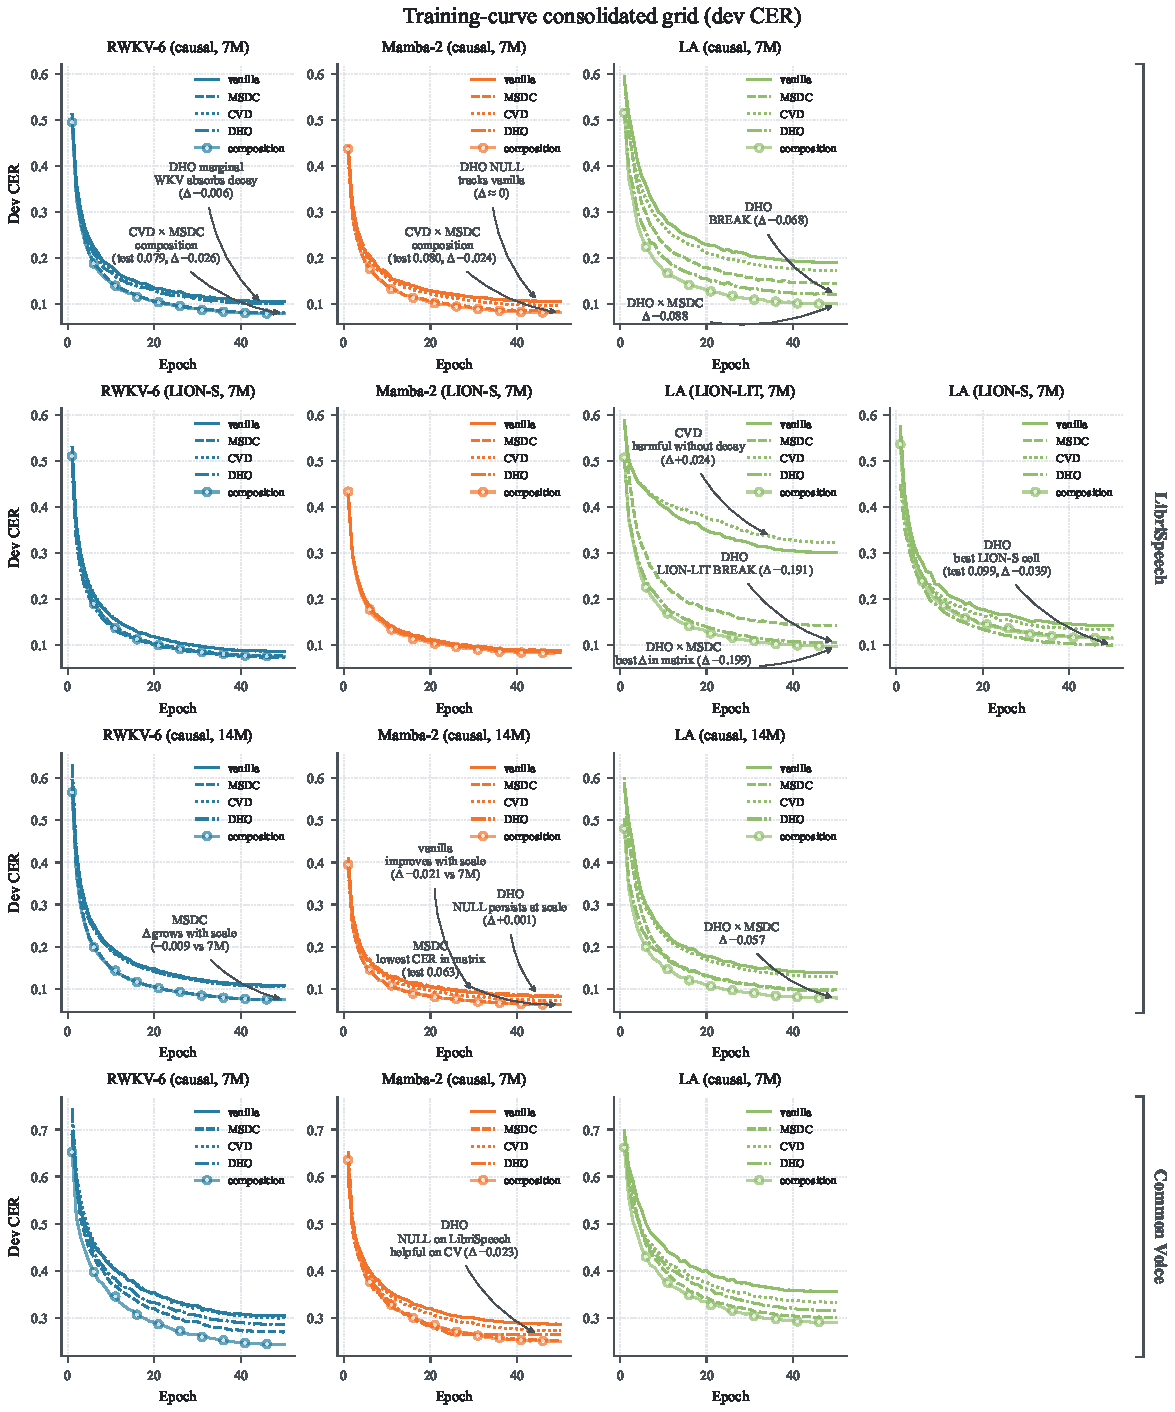
\includegraphics[width=0.95\linewidth]{chapter5/F11_training_curves.pdf}
\caption[Per-cell training curves]{Per-cell training curves on the
LibriSpeech matrix at the matched 50-epoch budget. Each panel is a
single cell; the y-axis is dev CER and the x-axis is epoch. The
patience-15 early stopping criterion is not triggered for any
reported cell within the 50-epoch horizon.}
\label{fig:app:training-curves}
\end{figure}
